\chapter{Concept and Design}
\label{cha:conceptanddesign}
 
The standards presented in \autoref{cha:relatedwork} show the potential improvements that can be achieved in key components of ActiviyPub-based social networks. In this section, we are going to go through the different steps that are required firstly to integrate DIDs into Mastodon, and finally to enable DIDComm for its communication. As explained in \autoref{cha:relatedwork}, Mastodon is the social network that pioneered the use of ActivityPub on a large scale, and it is also the social network with the most active users and presence inside the Fediverse. For this reason, the proposal presented in this section and the modus operandi of the ActivityPub server are going to be scoped to the actual implementation in Mastodon.\\
The outline for this chapter is the following. First, individual concepts of the ActivityPub implementation are explained. Then, an example of a simple use case in Mastodon's implementation is going to be illustrated and analyzed in order to be able to compare it with \autoref{section:did_flow}, which finally presents the same use case but with the proposed concept and design that includes DID integration and DIDComm enablement.
 
\section{Definitions}
Mastodon has implemented its own ActivityPub server, and with it also its own terms to express different social network vocabulary. In order to prevent confusion or ambiguities, the used terms in this chapter are explained here. 
 
\begin{itemize}
  \item \textbf{Username}: The username in Mastodon consists of a unique local username and the domain of the instance. Ex. alice@example.com
  \item \textbf{Actor object}: In this section, the term \emph{Actor object} refers solely to the ActivityPub's actor object. 
  \item \textbf{Toot}: In the user-facing part of Mastodon, a Toot is the äquivalent of a Tweet on Twitter. This is a small status update with a 500-character limit.
  \item \textbf{Status}: In the backend of Mastodon, the class used for a Toot is a Status. An account in Mastodon has a 1:n relationship with statuses.
\end{itemize}

\section{Use case}\label{section:use_case}
In order to explain the current ActivityPub flow in Mastodon, let's describe what happens in the simple use case:

\emph{Alice has an account in the Mastodon instance alice\_server.com and follows Bob, who has an account in the Mastodon instance bob\_server.com. Alice sends a direct message to Bob with the text: "Hello Bob!" }

\section{Mastodon's implementation}

\subsection{Activity creation}
The first thing that happens when Alice presses the send button is the creation of an ActivityStreams object. In this case, the object is of type \emph{Note} and will be created by Alice's server, as shown in \ref{fig:create_note}. Then, following the ActivityPub pattern of "some activity by some actor being taken on some object"\cite{lemmer-webber_tallon_guy_prodromou_2018}, the server wraps it in a \emph{Create} activity. The activity includes Alice in the \emph{attributeTo} field \ref{fig:create_activity}. Now that the actor, the activity, and the object are well defined and wrapped, it is time to shift our focus to the recipients of this note object. 
Alice's server will now look at the fields to, bto, cc, bcc, and audience to retrieve the recipients. Depending on where the recipient's account lives, the Alices' server may take one of two options. Nonetheless, the use case explicitly dictates that Bob's account resides in a different Mastodon instance, namely \emph{bob\_server.com}.

% Note Object with content: 'Hello Bob'
\lstset{style=JSONStyle}
\begin{lstlisting}[language=PHP, caption=ActivityStreams note object, label=fig:create_note]
  {
    "@context": "https://www.w3.org/ns/activitystreams",
    "type": "Note",
    "to": "http://bob_server.com/users/bob",
    "attributedTo": "http://alice_server.com/users/alice",
    "content": "Hello Bob!"
  }
\end{lstlisting}

\lstset{style=JSONStyle}
\begin{lstlisting}[language=PHP, caption=ActivityStreams create activity, label=fig:create_activity]
  {
    "@context": "https://www.w3.org/ns/activitystreams",
    "type": "Create",
    "id": "https://alice_server/users/alice/statuses/634367/activity",
    "to": "http://bob_server.com/users/bob",
    "actor": "http://alice_server.com/users/alice",
    "object": {
      "type": "Note",
      "to": "http://bob_server.com/users/bob",
      "attributedTo": "http://alice_server.com/users/alice",
      "content": "Hello Bob!"
    }
  }
\end{lstlisting}

\subsection{DNS-based Resolving Process}
If the recipient's account is on the same server, there is then no explicit resolving process. A simple query in the ActivityPub's server would find the right account and save the status within the account's statuses. On the contrary, when the recipient's account is not on the same server, then a resolving process must be started. Resolving is the fundamental part of the federated side of Mastodon. Without it, users within different instances would not be able to interact, as the instance itself does not know where to find the actor object with all required endpoints to send or receive activities from and to external accounts. For this reason, the current way to look up other accounts is through the DNS. In the same way Email works, the domain part of the username in Mastodon points to the domain of the instance where the account lives. The purpose of the resolving in this specific use case is to find the inbox URL of Bob, which can be found in Bob's actor object. As explained in \autoref{cha:relatedwork}, Mastodon includes a series of well-known endpoints that are used to retrieve information about resources managed by the host. As Bob's account lives inside \emph{bob\_server.com}, Mastodon triggers a Webquery request to bob's server Webquery endpoint. The request shown in \ref{fig:webfinger_request} will return a JRD Document, as shown in figure \ref{fig:webfinger_response}. Based on this document, Alice's server retrieves the link with the \emph{rel: 'self'} which includes the type and the URL where Bob's actor object can be retrieved. A subsequent HTTP GET request to this URL with the specific \emph{application/activity+json} header will return Bob's actor object. If the Webfinger request \ref{fig:hostmeta_request} returns a 404 code, it will then try, as a fallback, using the Host-Meta endpoint. The response constains a link template\ref{fig:hostmeta_response}, that Alice's server can use to try the Webquery request again.  

\begin{lstlisting}[language=PHP, caption=Webfinger request, label=fig:webfinger_request]
  GET /.well-known/webfinger?resource=acct:bob@bob_server.com HTTP/1.1
  Host: bob_server.com
  Accept: application/ld+json
\end{lstlisting}

\lstset{style=JSONStyle}
\begin{lstlisting}[language=PHP, caption=Webfinger response, label=fig:webfinger_response, float=h]
  {
    "subject": "acct:bob@bob_server.com",
    "aliases": [
      "https://bob_server.com/@bob",
      "https://bob_server.com/users/bob"
    ],
    "links": [{
        "rel": "http://webfinger.net/rel/profile-page",
        "type": "text/html",
        "href": "https://bob_server.com/@bob"
      },
      {
        "rel": "self",
        "type": "application/activity+json",
        "href": "https://bob_server.com/users/bob"
      },
      {
        "rel": "http://ostatus.org/schema/1.0/subscribe",
        "template": "https://bob_server.com/authorize_interaction?uri={uri}"
      }
    ]
  }
\end{lstlisting}

\begin{lstlisting}[language=PHP, caption=Hostmeta request, label=fig:hostmeta_request, float=h]
  GET /.well-known/host-meta HTTP/1.1
  Host: bob_server.com
  Accept: application/xrd+xml
\end{lstlisting}

\lstset{style=JSONStyle}
\begin{lstlisting}[language=PHP,caption=Hostmeta response, label=fig:hostmeta_response, float=h]
  <?xml version="1.0" encoding="UTF-8"?>
  <XRD xmlns="http://docs.oasis-open.org/ns/xri/xrd-1.0">
      <Link rel="lrdd" template="https://bob_server.com/.well-known/webfinger?resource={uri}"/>
  </XRD>
\end{lstlisting} 

\subsection{Delivery}
Succeeding the retrieval of Bob's actor object and therefore the needed inbox URL, the delivery can now take place. To provide end-to-end message integrity and to authenticate Alice in Bob's server, the request is signed by Alice's server using the HTTP Signature specification. Upon receiving the POST request to Bob's inbox URL, Bob's server has to verify the signature. For this, it starts the resolving process all over again to access the actor object of Alice, where Alice's public key can be found. After successful validation, Bob's server saves the Note object in Bob's statuses.
As indicated in \autoref{subsec:mastodon}, HTTP signatures are not part of the ActivityPub protocol standard. These security feature are within the Mastodon implementation of ActivityPub.

% Current Flow diagram
\begin{figure}[H]
  \centering
  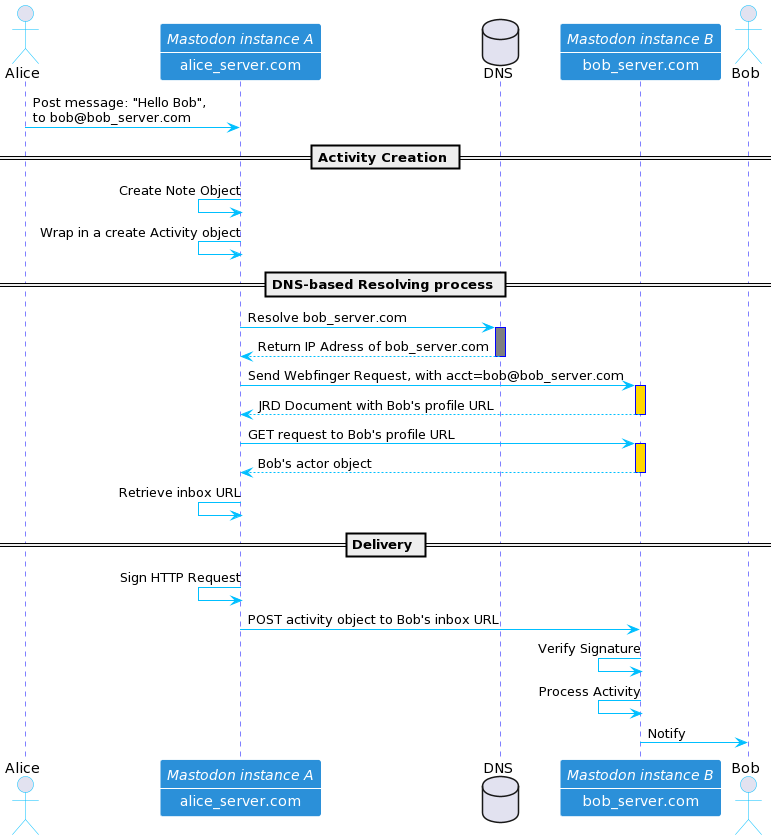
\includegraphics[width=\textwidth]{concept_and_design/normal_flow.png}
  \caption{Current flow for sending message}
  \label{fig:normal_flow}
\end{figure}

\pagebreak

% ------------Proposed Implementation------------------------------------
\section{Proposed implementation}\label{section:did_flow}
Having seen a state-of-the-art implementation of ActivityPub for our use case, it is now imperative to address the necessary steps to make ActivityPub DID-compliant, as well as enabling DIDComm as its communication protocol. 

\subsection{Requirements}
The proposed implementation wants to take advantage of the features provided by both DIDs and DIDComm, mentioned in \autoref{cha:relatedwork}. The following list of non-functional requirements derives of these advantages. 

\textbf{Requirement 1: Decentralization}
The design must be independent of any kind of centralized authority in trust encryption, as well as identifier and key management.

\textbf{Requirement 2: Private}
\textbf{Requirement 2: Private}
The design must allow users to control what information they want to disclose, and unauthorized third parties from learning who’s communicating about what

MUST preserve the integrity of messages against tampering; MUST allow the authenticity of messages and message senders to be proved; MUST use best-of-breed crypto; MUST allow parties to emit both repudiable and non-repudiable messages

Private (MUST prevent unauthorized third parties from learning who’s communicating about what, when; MUST give the sender the option to be anonymous to the recipient)
Decentralized (derives trust for encryption, signing, authn, and authz from control of decentralized identifiers rather than oracles like CAs, IDPs, etc; usable at the edge)
Transport-agnostic (usable over HTTPS 1.x and 2.0, WebSockets, BlueTooth, chat, push notifications, libp2p, AMQP, SMTP, NFC, sneakernet, snail mail; supports both simplex and duplex; works offline; doesn’t assume client-server or synchronous or real-time; allows paired or n-wise or public broadcast usage)
Routable (like email, Alice can talk to Bob without a direct connection to Bob; allows mixed and dynamic transports; passes through mix networks and other generic infrastructure that sees only payload BLOBs)
Interoperable (works across programming languages, blockchains, vendors, OS/platforms, networks, legal jurisdictions, geos, cryptographic schemes, and hardware — as well as across time; avoids vendor lock-in)
Extensible (lets developers start simple without heavy learning or dependencies; customizes easily; facilitates higher-level protocols that inherit DIDComm Messaging’s guarantees)
Efficient (doesn’t waste bandwidth, battery, storage space, or CPU)

\subsection{Implications of integrating DIDs}
The first question that needs to be addressed when approaching the integration of DIDs is, what are the implications of switching from standard mastodon usernames to DIDs. Integrating DID to ActivityPub points immediately to the actor's object, as the switch would mean that the DID has to be included somehow. Currently, most of the interactions of Mastodon via ActivityPub require the ID property to resolve to the user's profile to his actor's object. Following a simple strategy, we could simply replace the username with the DID. Thus having an ID like \verb|"www.alice_server.com/users/did:example:123456789abcdefghi"|.\\
However, there is another alternative that might work. Following the ActivityPub's specification, the ID must be a publicly dereferenceable URI, whose authority belongs to the originating server \cite{lemmer-webber_tallon_guy_prodromou_2018}. As explained in \autoref{section:dids}, a DID is a URI and it is publicly dereferenceable by nature. This allows different possibilities, to which the DID can be added. For example, using a stand-alone DID as an ID to take advantage of the discoverability of DIDs. This scenario would have the following implications. If another ActivityPub server wanted to get the user's profile URL, it would require resolving the DID to its respective DID document. This requires the DID document to include the actor's profile URL in the services section. Moreover, another option would be to add a DID URL with a query that points directly to the service endpoint that contains the actor's profile URL. Adding more precision, although still requiring a DID resolution as an intermediate step, as well as adding the service endpoint to the DID Document. Both cases are possible because ActivityPub has the \emph{URL} property that requires the actor's profile URL in case it is not in the ID property \cite{lemmer-webber_tallon_guy_prodromou_2018}. Although plausible, for this thesis a simple replacing strategy will be implemented, keeping the ID property as the profile's URL with the username replaced with the DID. \\
In addition to the ID, the actor's object must provide a supplementary set of URLs that point to different collections related to the user, as mentioned in \autoref{subsec:mastodon}. Following the same approach as with the ID, what if instead of using the actual URL of these collections, DID URLs pointing to the correct endpoint inside the DID Document were specified? An example for the inbox could be: \verb|"did:example:123456789abcdefghi#inbox"|.

This approach leads to the question, would it be simpler just to shift the whole actor object directly to the DID Document? This would imply that the actor object of ActivityPub is not necessary anymore and could be removed. This idea was briefly suggested by \cite{webber_sporny_2017} in a paper prepared for the 2017 Rebooting Web of Trust summit. Such an idea would look like fig. (DID Document with all ActivityPub endpoints). Furthermore, the authors went a step further and proposed cutting all dependency from the DNS by using onion websites. However, there are some security privacy concerns regarding the use of service endpoints in the DID Document that would advise against this. The DID specification stipulates \emph{"revealing public information through services, such as social media accounts, personal websites, and email addresses, is discouraged"} \cite{sporny_longley_sabadello_reed_steele_2021}. DID Documents are stored in a publicly available verifiable data registry, therefore any personal information revealed here is for everyone to see. The usage of URLs in service endpoints might lead to involuntary leakage of personal information or a correlation between the URL and the DID subject. Looking at figure \ref{fig:diddoc_related}, the amount of personal information displayed in the DID Document, which would not be otherwise inferable, already poses a privacy issue for the DID Subject. For this reason, in this thesis we differ from removing the actor's object from the ActivityPub protocol itself. This would also allow us to use freely all the other attributes in the actor's object to further describe its owner, such as name, preferredUsername, or summary without making this information forever public in an immutable ledger. Fig(final Actor'S object) illustrates the final design for the DID-compliant actor object. 

% \lstset{style=JSONStyle}
% \begin{lstlisting}[language=PHP,caption=DID document with ActivityPub actor, label=fig:diddoc_related, float=h]
%   {
%     "@context": ["https://example.org/did/v1",
%                  "https://www.w3.org/ns/activitystreams"],
%     "id": "did:example:d20Hg0teN72oFeo0iNYrblwqt",
%     "activityPubService": {
%       "id": "did:example:d20Hg0teN72oFeo0iNYrblwqt#services/ActivityPub",
%       // ActivityPub actor information
%       "type": "Person",
%       "name": "Alyssa P. Hacker",
%       "preferredUsername": "alyssa",
%       "summary": "Lisp enthusiast hailing from MIT",
%       "inbox": "https://9GaksjPhy0mWToTV.onion/alyssa/inbox/",
%       "outbox": "https://9GaksjPhy0mWToTV.onion/alyssa/outbox/",
%       "followers": "https://9GaksjPhy0mWToTV.onion/alyssa/followers/",
%       "following": "https://9GaksjPhy0mWToTV.onion/alyssa/following/",
%       "liked": "https://9GaksjPhy0mWToTV.onion/alyssa/liked/"},
%     // DDO information
%     "owner": [{
%       "id": "did:example:d20Hg0teN72oFeo0iNYrblwqt#key-1",
%       "type": ["CryptographicKey", "EdDsaPublicKey"],
%       "curve": "ed25519",
%       "expires": "2017-02-08T16:02:20Z",
%       "publicKeyBase64": "lji9qTtkCydxtez/bt1zdLxVMMbz4SzWvlqgOBmURoM="
%     }, {
%       "id": "did:example:d20Hg0teN72oFeo0iNYrblwqt#key-2",
%       "type": ["CryptographicKey", "RsaPublicKey"],
%       "expires": "2017-03-22T00:00:00Z",
%       "publicKeyPem": "----BEGIN PUBLIC KEY-----\r\n.."
%     }],
%     "control": [{
%       "type": "OrControl",
%       "signer": [
%           "did:example:d20Hg0teN72oFeo0iNYrblwqt",
%           "did:example:8uQhQMGzWxR8vw5P3UWH1j"
%       ]
%     }],
%     "created": "2002-10-10T17:00:00Z",
%     "updated": "2016-10-17T02:41:00Z",
%     "signature": {
%       "type": "RsaSignature2016",
%       "created": "2016-02-08T16:02:20Z",
%       "creator": "did:example:8uQhQMGzWxR8vw5P3UWH1j#key/1",
%       "signatureValue": "IOmA4R7TfhkYTYW8...CBMq2/gi25s="
%     }
%   }
% \end{lstlisting} 

% --- Mastodon implementation -----
Regarding Mastodon, replacing the standard username with a DID does not imply huge complications. The way Mastodon validates the username format is through the following regular expression: 

\begin{verbatim}
  USERNAME_REGEX = /[a-z0-9_]+([a-z0-9_\.-]+[a-z0-9_]+)?/i
\end{verbatim}

Additionally, it has a length constraint of 30 characters. The following DID-syntax-compliant regular expression can be used instead, as well as an extended maximum length of 85 characters. 

\verb|DID_REGEX = /did+:+[a-z0-9_]+([a-z0-9_\.-]+[a-z0-9_]+)?:|\\\verb|[A-Za-z0-9\.\-\:\_\#]+/i |


\subsection{Decentralized resolving process}
As stated in the previous section, Mastodon starts the resolving process based on the username of the user. By replacing the standard username with a DID, the current resolving flow gets disrupted, as there is no domain and thus no well-known endpoints to send requests to. Nonetheless, here is where the resolvability of the DIDs come into play. The proposed flow takes the following steps. Firstly, the username, which now is a DID, can be resolved to its DID Document using any kind of DID resolver. The DID Document must now contain a service with the type ActivityPub and an endpoint, where the actor's object can be retrieved. This gives us 2 possibilities. On the one hand, we could add in the well-known Webfinger endpoint, which then provides us with the profile URL from the user. On the other hand, we could skip the Webfinger request and provide the profile URL directly in the DID Document. The latter looks like the most meaningful path to take. Especially when we refer to the purpose of Webfinger, which was to enable discoverability of entities represented by URIs \cite{jones_salgueiro_jones_smarr_2013}. Webfinger's purpose shares a lot of ground with the design of DIDs, nevertheless, the DID design provides a less limited structure of resolving, as it does not rely on DNS and HTTP for its functioning. For this reason, the proposed workflow will completely remove the use of the  Webfinger protocol used in Mastodon and include the URL of the user's profile in the ActivityPub service section in the DID Document.

The easiest way to set a DID resolver, is to use the one from the DIF. They provide Docker images for the service running the query endpoint, and for the drivers needed for each DID method. As Mastodon can be run using Docker Compose, the resolver can be added to the same docker network as the main backend application. This would allow accessing the resolver through the alias name \emph{did-resolver}. The resolver validates the DID document by comparing the searched DID against the ID attribute of the DID document and only returns the DID document when both match. To make the requests to the resolver the service class \emph{DidResolverService} will be added to the backend. The only parameter it needs is the DID it needs to resolve, and it returns the DID Document as a JSON object. Furthermore, to facilitate the interaction with the properties of the DID document a class \emph{DidDocument} with the methods listed in table \ref{table:did_doc_instance_methods} is also needed.

\begin{table}[!ht]
	\centering
	\begin{tabular}{| l | l | l |}
		\hline
    Function & Description \\
		\hline
		\hline
      initialize(attributes) &  Stores the attributes of the DID document in accesible variables\\
    \hline
      serviceEndpoint & Returns the service endpoint URL of the first service \\
    \hline
      didcommKey & Looks for a specific key in the \\ & DID document and returns a parsed instance of it \\
    \hline
	\end{tabular}
	\caption{DID document instance methods}
  \label{table:did_doc_instance_methods}
\end{table}

With DIDs, a resolver, and a class for DID documents set up, the next task is to modify the Webfinger-based resolving process of Mastodon. Mastodon has a class called \emph{ResolveAccountService}, which triggers the Webfinger requests and processes the respective responses. It takes a username in the form of \emph{username@domain} as a parameter. If the username does not have an existing account in the local database, it makes the Webfinger request. The JRD response gets parsed to find the actor URL, and a subsequent request to the username domain gets triggered to get the actor object. Finally, it parses the actor object to create an account for this user in the local database.
The new class handling the decentralized DID-based resolving process is not very different. It also takes the username parameter in the form of \emph{did:method:example} and then uses the resolver service to make a query to the universal resolver. A \emph{DidDocument} class gets created with the JSON response and the actor URL its obtained using the \emph{serviceEndpoint} method. Finally, as in the previous flow, a request is made to this URL to get the actor object for further processing.

\subsection{Enabling DIDComm Messaging}\label{section:enabling_didcomm}

Having introduced DIDs to Mastodon and ActivityPub, it is now possible to enable DIDComm. Taking into account the algorithm \ref{alg:didcomm_example} shown in \autoref{section:didcomm}, it is possible to derive some requirements that DIDComm imposes:

\textbf{1. Access to private key}: The ActivityPub server requires access to the private key of the selected verification method. Furthermore, the ActivityPub server must be able to support the keys and the cryptographic algorithms, which the JWA includes. This means having any library that can parse them and perform encryption and decryption with them.

\textbf{2. Key agreement}: DID Documents may present more than one verification method specified in them. A specific standard verification method is required to maintain compatibility between the parties involved. This means that the sender and the recipient must use the same set of keys for encryption and/or signing purposes to have a successful message exchange through DIDComm. The DID specification luckily provides us with a recommendation for this. The \emph{keyAgreement} verification relationship is intended to provide the keys, which allows an entity to confidentially share information with the DID-subject using encryption \cite{sporny_longley_sabadello_reed_steele_2021}. Even though it is possible to add an extra verification relationship called DIDComm or ActivityPub that works in conjunction with our previously defined ActivityPub service, we will stick to the recommendation using the \emph{keyAgreement} key for this proposal.

\textbf{3. Access to DID-Resolver}: This is for cases where a signature needs to be verified using an external public key. However, this requirement has already been fulfilled. 

Creating a DID is rather a simple task. However, finding a DID method that would allow CRUD operations to add the service endpoint and a \emph{keyAgreement} key to its DID Document without needing to pay any GAS or any other kind of fees is not. The following options were tested. MATTR\footnote{https://mattr.global}offers creating DIDs using \emph{did:key}, \emph{did:web} and \emph{did:ion} methods. However, they do not allow creating own keys or accessing private keys, which is necessary according to the first requirement. \emph{did:ion} offers a set of tools\footnote{https://github.com/decentralized-identity/ion-tools} to perform CRUD operations in a self-created DID and DID document. These tools are bundled in a library called ION.js, which wraps the SDK and provides an interface to interact easily with the components of ION. However, even though the \emph{update} operation is allowed, it was not possible to fetch a previously created DID and then update it, which was a necessary step. More users have encountered this issue\footnote{https://github.com/decentralized-identity/ion-tools/discussions/25}, but so far, it has not been addressed by the developers. An alternative to ledger-based DIDs developed for this thesis was using the \emph{did:web} method. This method allows hosting the DID Document on any server, giving the server-owner full control. Nonetheless, the discovery process of this type of DID relies heavily on DNS because the DID resolver makes a GET request to the \emph{.well-known/did} endpoint of the domain in the DID to retrieve the DID document. This dependency on the domain would prevent achieving the goal of independence of centralized services. \\
Another DID method researched was the Uport-developed \emph{did:ethr}. Uport is now divided into two projects, namely Serto\footnote{https://serto.id} and Veramo\footnote{https://veramo.io}. Each one of them offers a decentralized identity solution. On the one hand, Serto provides a platform in the AWS Marketplace that can be easily deployed and would allow a user to create and manage DIDs from the \emph{did:ethr} method. Unfortunately, after failing to deploy the EC2 instance and contacting Serto's developers, it turned out it was temporarily not working. On the other hand, Veramo's typescript-based API allows users to manage DIDs not only in the Ethereum main network but also in other test networks such as Ropsten and Rinkeby. This allows making CRUD operations to DIDs without incurring costs. Veramo provides a setup guide\footnote{https://veramo.io/docs/node\_tutorials/node\_setup\_identifiers}, where the only thing needed externally is an Infura\footnote{https://infura.io} account to use as a Web3 Provider. Two DIDs were created in the Ropsten network for Alice and Bob, respectively.

\begin{itemize}
  \item \textbf{Alice:} 
  did:ethr:ropsten:0x031be4622770a8ee4a7b25d1673e829fd2eb5f4762efcb18d09d468\\e6a00cc6c4d
  \item \textbf{Bob:} 
did:ethr:ropsten:0x03117951c6011b4a46f11a67fc7f67f746a7ad84daaae69623db833d\\dd56397c37
\end{itemize}

Having DIDs created, the next task is to add the ActivityPub service endpoint to the DID documents of Bob and Alice. The parameters required for Veramo's API to process the information correctly, as shown in figure \ref{fig:add_service_payload}, are the DID, the service, and options for the Web3 provider. The service includes must have a type, a service endpoint, and a description. A service's id is optional, as the Web3 Provider will overwrite it. 

\lstset{style=JSONStyle}
\begin{lstlisting}[language=PHP, caption=Parameters to add a service in Veramo, label=fig:add_service_payload, float=h]
  const service_args= {
    did: <alice DID>,
    service: {
      id: 'ActivityPub', // This field will be overwritten
      type: "ActivityPub",
      serviceEndpoint: "http://alice_server.com/users/" + <alice DID>,
      description: "DIDComm enabled ActivityPub Actor"
    },
    options: {
      gas: 100_000, // between 40-60000
      ttl: 60 * 60 * 24 * 365 * 10 // make the service valid for ~10 years
    }
  }
\end{lstlisting}

The biggest challenge in implementing DIDComm is the compatibility between the algorithms specified by the JWA spec, the key types, and the libraries used to generate keys, sign, and encrypt. In Mastodon, OpenSSL\footnote{https://github.com/ruby/openssl} is the library used for generating the RSA keys used for the HTTP and JSON-LD signatures. This library wraps the OpenSSL project toolkit\footnote{https://www.openssl.org/} and provides a wide range of key management, encryption, decryption, and certificates management. To create signed and encrypted messages, the JWT library\footnote{https://github.com/jwt} for ruby on rails was selected as it allows the spec-compliant creation of JWS and JWE tokens.\\
For this proposal, the objective is to add confidentiality, integrity, and non-repudiation to every ActivityPub object sent in Mastodon. As explained in \autoref{section:didcomm}, the recommended way to achieve this is by using \emph{authcrypt}. However, during the development of this thesis, there were no libraries for Ruby and Rails that supported the \emph{ECDH-1PU} algorithm. Furthermore, the JWT library had a limited number of available algorithms. For this reason, it was decided to implement a nested JWT, following the same procedure as algorithm \ref{alg:nested_jwt}. To prevent any further compatibility problems on the key generation side, it was decided to use the common widely-supported RSA key generation algorithm. This means, that both Alice and Bob will have an extra RSA keypair, and the private keys will be stored in their respective Mastodon instance. The JWS tokens were set to use an RSA 2048 key and the \emph{RS256} hash algorithm, and the JWE tokens to use the \emph{RSA-OAEP}\footnote{https://www.rfc-editor.org/rfc/rfc7518\#page-14} algorithm for key management with the \emph{A128CBC-HS256}\footnote{https://www.rfc-editor.org/rfc/rfc7518\#page-22} algorithm for encryption.
With existing RSA keys for both our actors, it is now necessary to add the respective public keys to their DID documents. Veramo's API offers a way to add different kinds of cryptographic keys to a DID document, however, the only available key types that could be added were the \emph{Ed25519}, \emph{Secp256k1}, and the  \emph{X25519} from the \emph{Elliptic Curve Cryptography} (ECC) family of cryptosystems. This represented a considerable complication, as the already mentioned library for the JWT tokens did not have support for these types of keys. Luckily, after researching possible workarounds, one of the main developers of the Veramo project assisted and developed a way to \emph{force} adding an RSA key to the DID document. The final DID document for Alice's DID can be seen in figure \ref{fig:alice_ethr_doc}.

% \lstset{style=JSONStyle}
% \begin{lstlisting}[language=PHP, caption=\emph{did:ethr} DID document with added RSA verification method and ActivityPub service endpoint in the mastodon instance \emph{lisztos.com}, label=fig:alice_ethr_doc, float=h]
%   {
%   "@context": [
%     "https://www.w3.org/ns/did/v1",
%     "https://w3id.org/security/suites/secp256k1recovery-2020/v2"
%   ],
%   "id": "did:ethr:ropsten:0x031be4622770a8ee4a7b25d1673e829fd2eb5f4762efcb18d09d468e6a00cc6c4d",
%   "verificationMethod": [
%     {...},
%     {
%       "id": "did:ethr:ropsten:0x031be4622770a8ee4a7b25d1673e829fd2eb5f4762efcb18d09d468e6a00cc6c4d#delegate-1",
%       "type": "RSAVerificationKey2018",
%       "controller": "did:ethr:ropsten:0x031be4622770a8ee4a7b25d1673e829fd2eb5f4762efcb18d09d468e6a00cc6c4d",
%       "publicKeyPem": "-----BEGIN PUBLIC KEY-----\nMIIBIjANBgkqhkiG9w0BAQEFAAOCAQ8AMIIBCgKCAQEAspiTbG8OCy39BvI0rnTH\nVGEW2YpYTs+ayH9FtmyTdeHifIJLF0breFsKAM/HE8EQF3iI4tjMYI5c1A04FLRY\ncmwLRkNGlv8+2seCFoN+Hkv+5eupjkr+x32amvmbB92B3s7oqW5IftveAnxWJPEi\nY1Fm3tGiYz85Yg+3IOEp9083IKaZu1visW1Sp0YObwZLJCNzE6o3bOfpKMSBkzoc\nmBxkFXD0ilmXqM2CETsYfaywFachOu1dC+XcF/npUZV+Q1FdWLiuFlKAwDt3DiD3\nNSz2b27Iga7wTSCoQ/DAhFAZ8KH8uCMrioIWFSKuYRgFOysbDfTT9Kpha8ST8K/H\nTQIDAQAB\n-----END PUBLIC KEY-----\n"
%     }
%   ],
%   "authentication": [...],
%   "assertionMethod": [...],
%   "service": [
%     {
%       "id": "did:ethr:ropsten:0x031be4622770a8ee4a7b25d1673e829fd2eb5f4762efcb18d09d468e6a00cc6c4d#service-1",
%       "type": "ActivityPub",
%       "serviceEndpoint": "http://lisztos.com/users/did:ethr:ropsten:0x031be4622770a8ee4a7b25d1673e829fd2eb5f4762efcb18d09d468e6a00cc6c4d"
%     }
%   ]
% }
% \end{lstlisting}


At this point, all the elements needed to enable DIDComm are present, i.e. two Mastodon instances for federated communication with DID integration, a DID resolver and a service class that can resolve DIDs, as well as DID documents for both actors with the ActivityPub service endpoint and the public key for the verification method. The next step is to put them together. As part of this proposal, further changes to the ActivityPub protocol itself are not in the scope. However, extending it and removing the dependency on the HTTP protocol for its communication is still intended. Therefore, encapsulation rather than modification of ActivityPub within DIDComm allows for a modular approach that keeps both protocols independent from each other. The simplest way to keep a modular approach is by using the ActivityStream object as a payload for our JWM, which would look like figure \ref{fig:jwm_example}. 
The final payload that will be sent in server-to-server communication will consist of a JWE token, whose content is a signed JWM that includes the Activity in its body, following the structure of figure \ref{fig:final_env}.

\lstset{style=JSONStyle}
\begin{lstlisting}[language=PHP, caption=JWM example, label=fig:jwm_example, float=h]
  {
    "id": "https://alice_server/users/did:example:alice/statuses/634367/activity",
    "type": "https://www.w3.org/ns/activitystreams",
    "body": {
      "@context": "https://www.w3.org/ns/activitystreams",
      "type": "Create",
      "id": "https://alice_server/users/did:example:alice/statuses/634367/activity",
      "actor": "https://alice_server.com/users/did:example:alice",
      "to": [ 
            "https://bob_server.com/users/did:example:bob"
        ],
      "object": {
        "type": "Note",
        "to": [ 
            "https://bob_server.com/users/did:example:bob"
        ],
        "attributedTo": "https://alice_server.com/users/did:example:alice",
        "content": "Hello Adrian!"
      }
    }
  }
\end{lstlisting}

\begin{figure}[h]
  \centering
  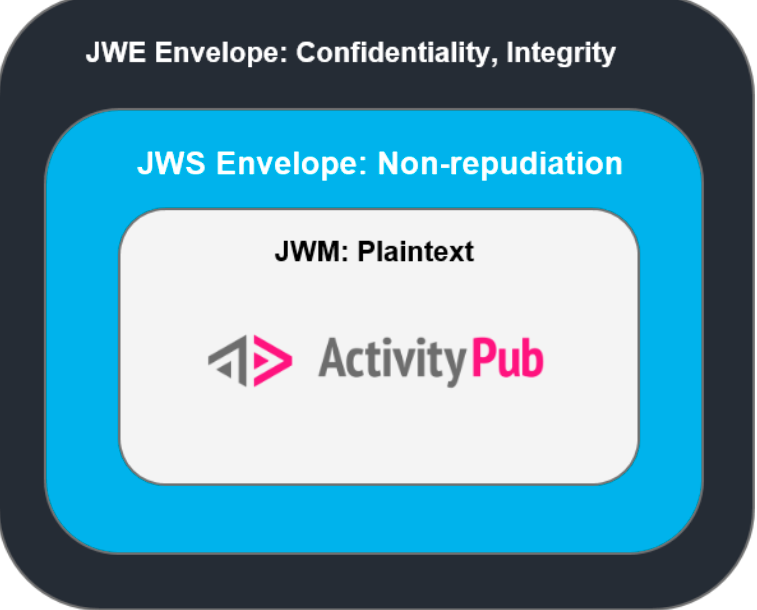
\includegraphics[width=0.5\textwidth]{concept_and_design/final_env.png}
  \caption{Proposed Payload structure using DIDComm and ActivityPub}
  \label{fig:final_env}
\end{figure}

The final flow for our use case mention in\ref{section:use_case} is illustrated in figure \ref{fig:did_flow}

% Proposed Flow diagram
\begin{figure}[h]
  \centering
  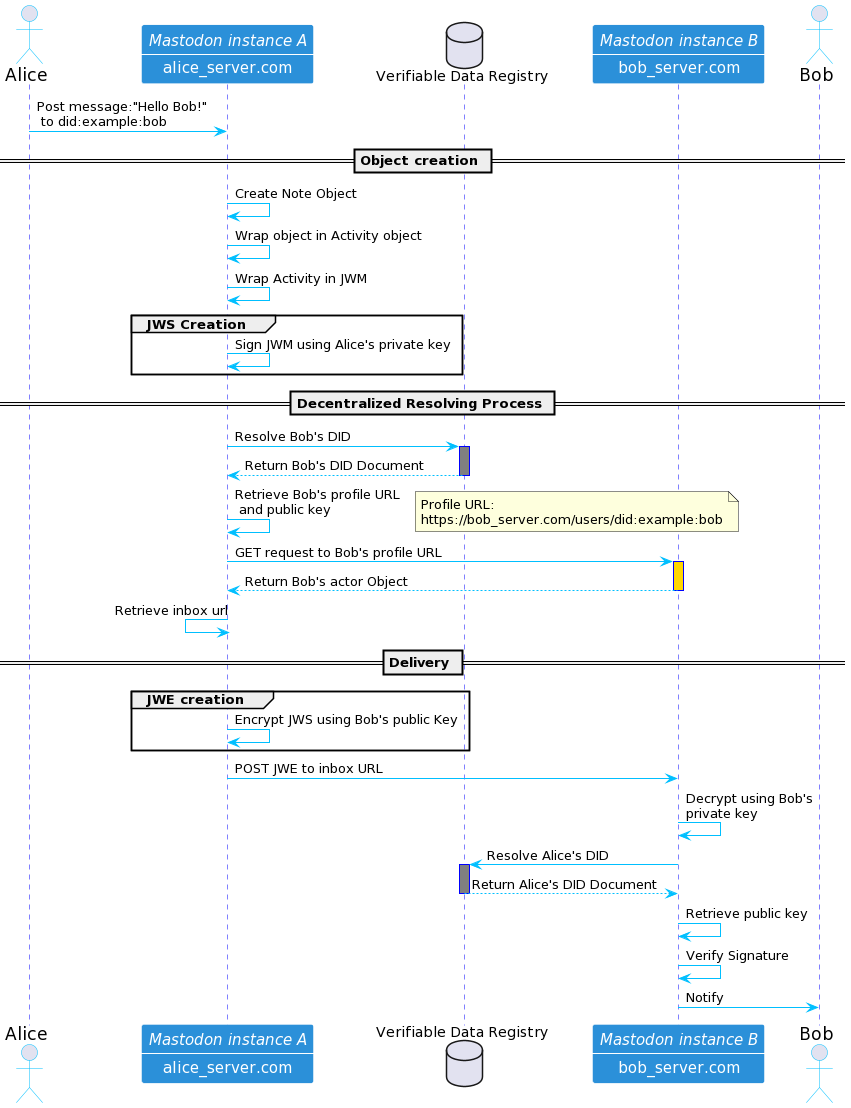
\includegraphics[height=\textheight, width=\textwidth]{concept_and_design/did_flow.png}
  \caption{DID and DIDComm flow for use case}
  \label{fig:did_flow}
\end{figure}



%
% -------DID Flow-------------
% @startuml

% skinparam backgroundColor White

% skinparam sequence {
% ArrowColor DeepSkyBlue
% ActorBorderColor DeepSkyBlue
% LifeLineBorderColor blue
% LifeLineBackgroundColor #2b90d9

% ParticipantBorderColor White
% ParticipantBackgroundColor #2b90d9
% ParticipantFontName Impact
% ParticipantFontSize 15
% ParticipantFontColor White

% ActorFontSize 17
% ActorFontName Aapex

% }
% actor Alice as a

% participant as [
%     ====Mastodon instance A
%     ----
%     alice_server.com
% ]
% database "Verifiable Data Registry" as VDR
% participant bs [
%     ====Mastodon instance B 
%     ----
%     bob_server.com
% ]
% participant "Bob's server" as bs
% actor Bob as b

% a->as:  Post message:"Hello Bob!" \n to did:example:bob

% == Object creation ==

% as->as: Create Note Object
% as->as: Wrap object in Activity object
% group JWS
% as->as: Wrap Activity in JWM
% as->as: Sign using Alice's private key
% end

% == Resolving Process ==
% as->VDR ++ #gray: Resolve Bob's DID
% VDR-->as --: Return Bob's DID Document
% as->as: Retrieve Bob's profile URL \n url and public key 
% note right
% Profile URL: 
% https://bob_server.com/users/did:example:bob
% end note
% group JWE
% as->as: Encrypt JWS using\nBob's public Key
% end group
% as->bs ++ #gold: GET request to Bob's profile URL
% bs-->as --: Return Bob's actor Object
% as<-as: Retrieve inbox url

% == Delivery ==
% as->bs: POST JWE to inbox url

% bs->bs: Decrypt using Bob's\nprivate key
% bs->VDR ++ #gray: Resolve Alice's DID
% VDR-->bs --: Return Alice's DID Document

% bs->bs: Retrieve public key 
% bs->bs: Verify Signature

% bs->b: Notify

% @enduml

% -------Normal Flow-------------

% @startuml

% skinparam backgroundColor White

% skinparam sequence {
% ArrowColor DeepSkyBlue
% ActorBorderColor DeepSkyBlue
% LifeLineBorderColor blue
% LifeLineBackgroundColor #2b90d9

% ParticipantBorderColor White
% ParticipantBackgroundColor #2b90d9
% ParticipantFontName Impact
% ParticipantFontSize 14
% ParticipantFontColor White

% ActorFontSize 14
% ActorFontName Aapex

% }
% @startuml
% actor Alice as a
% participant as [
%     ====Mastodon instance A 
%     ----
%     alice_server.com
% ]
% database DNS
% participant bs [
%     ====Mastodon instance B 
%     ----
%     bob_server.com
% ]

% actor Bob as b

% a->as: Post message: "Hello Bob",\nto bob@bob_server.com

% == Activity Creation ==

% as<-as: Create Note Object
% as<-as: Wrap in a create Activity object

% == Resolving process ==


% as->DNS ++ #gray: Resolve bob_server.com
% DNS-->as --: Return IP Adress of bob_server.com

% as->bs ++ #gold: Send Webfinger Request, with acct=bob@bob_server.com
% bs-->as --: JRD Document with Bob's profile URL

% as->bs ++ #gold: GET request to Bob's profile URL
% bs-->as --: Bob's actor object
% as<-as: Retrieve inbox URL

% == Delivery ==
% as<-as: Sign HTTP Request
% as->bs: POST activity object to Bob's inbox URL
% bs<-bs: Verify Signature
% bs<-bs: Process Activity
% bs->b: Notify

% @enduml








% Even though there are cases when very similar domains may lead to confusion and may present some security issues. Examples of this can be found simply by comparing the most used Mastodon instance “mastodon.social” with another big\\-in\-user\-count instance such as “mstdn.social”. This type of username allows the following scenarios to play out, where differences are minimal and easily missed out, such as alice@mastodon.social and alice@mstdn.social. In addition, some users have commented that when the username is too long, the domain is not longer visible. This can be exploited by malicious actors, who may open an account in a different server with the same username as their target. Clone their profile, and try to social engineer the target's followers. 

% \lstset{style=JSONStyle}
% \begin{lstlisting}[language=PHP, caption=Alice's actor object, label=fig:alice_actor_object, float=h]

% {
% 	"@context": [
% 			"https://www.w3.org/ns/activitystreams",
% 			"https://w3id.org/security/v1",
% 	],
% 	"id": "http://alice_server.com/users/alice",
% 	"type": "Person",
% 	"following": "http://alice_server.com/users/alice/following",
% 	"followers": "http://alice_server.com/users/alice/followers",
% 	"inbox": "http://alice_server.com/users/alice/inbox",
% 	"outbox": "http://alice_server.com/users/alice/outbox",
% 	"featured": "http://alice_server.com/users/alice/collections/featured",
% 	"featuredTags": "http://alice_server.com/users/alice/collections/tags",
% 	"preferredUsername": "alice",
% 	"name": "",
% 	"summary": "",
% 	"url": "http://alice_server.com/@alice",
% 	"manuallyApprovesFollowers": false,
% 	"discoverable": false,
% 	"published": "2022-06-14T00:00:00Z",
% }


% \end{lstlisting}

% As explained in \autoref{section:didcomm}, the JWM specification defines a series of attributes that provide a starting point for the use of JWMs. Not all of these are mandatory and can thus be modified depending on the use being given to them. This gives us a lot of room to think about what is necessary and what is not. As seen in fig. (JWM with activity), redundancy can be found in each level of the JSON object. For example, the sender and recipient are defined in each layer. In the end, the Activity is the only object that will be processed, therefore, the JWM does not necessarily need any extra information, because the Activity has already all the necessary information. Furthermore, even if we wanted to use the routing mechanism of DIDComm, the attributes From and To in the JWM would only be necessary in cases where we want to send plain text messages. In addition, in almost every case the message is being sent to a specific URL, like the inbox of another user. So the receiver server will always know to whom the Activity was directed. This leaves us with a JWM structure with the attributes id and type. The requiredness of these two differs from the JWM specification and DIDComm. Nonetheless, we will stick to DIDComm and keep these two attributes compulsory. The type should be a message type URI, therefore we will use the ActivityStreams schema URI, and for the ID, we will reuse the status ID. The result is shown by figure \ref{fig:jwm_example}